\subsection{Pouvoir séparateur de l'oeil}

\paragraph{Analyse de la précision et limites théoriques}
Le pouvoir séparateur moyen mesuré ($10^{-3} \mathrm{~rad}$) reste supérieur à la limite théorique de l'œil humain ($3 \cdot 10^{-4} \mathrm{~rad}$). 
Cette différence pourrait s'expliquer par un protocole expérimental dont l'incertitude est difficile à quantifier :
\begin{itemize}
    \item \textbf{Imprécision du déplacement} : La méthode consistant à reculer jusqu'à la disparition du contraste ("grisement") manque de résolution. Un pas humain représente une variation de distance d'environ $0,5 \mathrm{~m}$, ce qui induit une incertitude non négligeable sur la mesure de $D_m$.
    \item \textbf{Conditions lumineuses} : L'expérience s'est déroulée dans une pièce peu éclairée. Or, une faible luminosité provoque une dilatation de la pupille (mydriase), ce qui augmente les aberrations géométriques de l'œil et dégrade le pouvoir séparateur.
    \item \textbf{Facteur physiologique} : Sans doute que la fatigue oculaire des observateurs au moment de la mesure pourrait également expliquer l'écart avec les valeurs standards.
\end{itemize}

\paragraph{Pistes d'amélioration du protocole}
Pour affiner ces résultats, plusieurs modifications du protocole pourraient être envisagées :
\begin{itemize}
    \item \textbf{Optimisation de la mesure de distance} : Remplacer le déplacement libre par un système de repérage spatial plus stable (utilisation d'une chaise par exemple pour faciliter le repérage dans l'espace) pour permettre des mesures au centimètre près.
    \item \textbf{Contrôle de l'environnement} : Réaliser l'expérience sous un éclairage normalisé et constant pour stabiliser le diamètre pupillaire des observateurs.
    \item \textbf{Répétabilité} : Effectuer une série de mesures à différents moments de la journée pour moyenner l'impact de la fatigue visuelle.
\end{itemize}

\subsection{Diamètre et position du cercle oculaire}

Le diamètre du cercle oculaire mesuré ($1,5\mathrm{~mm}$) est en adéquation avec les données théoriques et biologiques. En effet, la pupille humaine en myosis (luminosité normale à forte) présente un diamètre d'environ $2\mathrm{~mm}$. Cette dimension garantit que l'intégralité du faisceau émergent du microscope pénètre dans l'œil de l'observateur, optimisant ainsi la clarté de l'image.

\paragraph{Analyse critique}
Bien que les mesures soient cohérentes avec l'usage standard de l'instrument, 
une démonstration rigoureuse par le calcul (formules de conjugaison ou de Newton) 
de la position et du diamètre théoriques s'avère complexe (car nous manquons de temps pour pousser plus loin l'analyse). 

\subsection{Discussion sur l'identification biologique}

\begin{figure}[h]
    \centering
    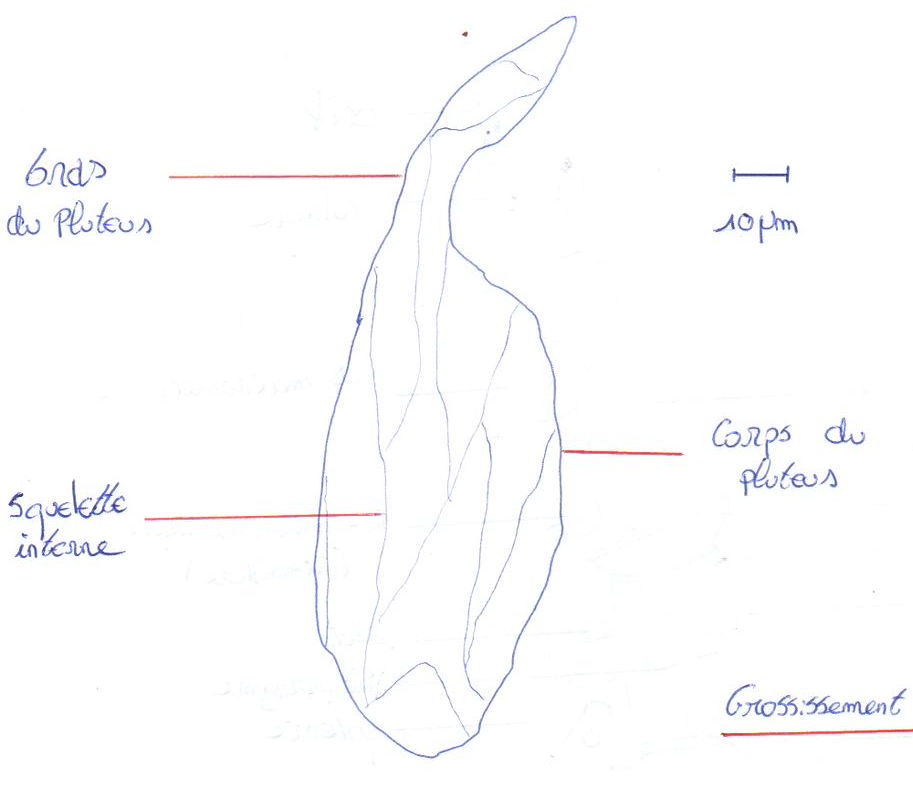
\includegraphics[width=0.6\textwidth]{figures/pluteus.jpeg} 
    \caption{Dessin d'observation d'un ovocyte (pas de larve !) d'oursin (Objectif $\times 10$). 
             Diamètre moyen estimé : $60\mathrm{~\mu m}$.}
    \label{fig:dessin_oeuf}
\end{figure}

Une analyse a posteriori des dimensions relevées 
soulève une interrogation sur la nature exacte de l'échantillon observé.

\paragraph{Analyse dimensionnelle}
Bien que l'échantillon ait été initialement identifié comme une larve Pluteus dans le fascicule, 
les mesures obtenues (entre $40\mathrm{~\mu m}$ et $80\mathrm{~\mu m}$) 
sont significativement inférieures aux standards biologiques d'une larve à ce stade, 
qui mesure classiquement entre $300\mathrm{~\mu m}$ et $500\mathrm{~\mu m}$.

\paragraph{Hypothèse de l'ovocyte}
Ces dimensions correspondent en revanche plutôt 
à l'ordre de grandeur d'un ovocyte d'oursin ($70$ à $100\mathrm{~\mu m}$). 

\paragraph{Conclusion sur la mesure}
Cette confusion d'identification n'entache cependant pas 
la validité de la manipulation physique en elle-même. 
Elle questionne tout de même sur la nécessité de bien comprendre ce que l'on 
cherche à identifier avant tout. 